\documentclass[11pt,a4paper]{ipmu}

% Packages
\usepackage{natbib}     % For bibliography
\usepackage{caption}    % Better control of figure captions
\usepackage{subcaption} % Subfigures
\usepackage{aas_macros}
\usepackage{rotating}   % For rotating figures
\usepackage{booktabs}
\usepackage{enumitem}
\usepackage{comment}

% Set Thesis Metadata
\setThesisTitle{Effects of Replicated N-body Simulation Boxes \\in Simulating Weak Lensing Observables}
\setThesisJapaneseTitle{弱重力レンズ統計量の模擬データ生成における\\有限体積のN体シミュレーションの影響の研究}
\setThesisAuthorEnglish{Akira Tokiwa}
\setThesisAuthorJapanese{常盤 晟}

\begin{document}

% Create Title Page
\makethesistitle

% Create Abstract Page
% \begin{abstractpage}
%     We investigate the influence of super-sample covariance on the covariance and correlation matrices of the power spectrum and higher-order statistics using two distinct simulation approaches: BIGBOX and TILED. Leveraging 11 realizations of state-of-the-art BIGBOX simulations from the HalfDome project, each containing $6144^3$ particles within a 3750 Mpc/h volume, and 20 TILED realizations composed of smaller $1024^3$-particle boxes within 625 Mpc/h, we analyze the convergence field under the Born approximation. Uniformly covering the full sky with $10^\circ \times 10^\circ$ patches extracted via a Fibonacci grid, we employ a comprehensive suite of higher-order statistics, including bispectrum, probability distribution function, peak and minima counts, and Minkowski functionals, and the angular power spectrum to probe the non-Gaussian features of the convergence maps.

Our comparative analysis reveals that mean statistical measures between BIGBOX and TILED simulations agree within 1\% across all statistics, redshifts, and multipoles, validating the simulations' reliability in capturing the underlying cosmological model. However, variance ratios exhibit significant differences of 10-30\%, particularly at high multipoles and redshifts, attributable to super-sample covariance arising from large-scale modes present in BIGBOX but absent in TILED. Shape noise impacts statistical measures, especially the angular power spectrum and peak/minima counts, yet super-sample covariance remains the dominant effect. Additionally, Gaussian smoothing affects small-scale features without substantially variating the covariance and correlation structures, while box replication artifacts introduce systematic biases by underestimating mean angular power spectra and distorting higher-order statistics.

These findings underscore the critical role of super-sample covariance in high-precision cosmological analyses, particularly for upcoming weak lensing surveys such as LSST, Euclid, and Roman. Accurate variance modeling necessitates the inclusion of large-scale modes in simulations, while maintaining robustness against shape noise and smoothing operations. Addressing systematic challenges like box replication artifacts is essential to prevent biases in the interpretation of higher-order statistics. Future work will focus on mitigating replication artifacts, incorporating diverse cosmological models and baryonic effects, and integrating these insights into survey design and data analysis pipelines to enhance the precision of cosmological parameter inference. Our study advances simulation techniques and observational strategies, reinforcing weak lensing as a pivotal tool for probing the Universe's fundamental properties with unprecedented accuracy.
% \end{abstractpage}

\tableofcontents  % Generates the table of contents
\listoffigures    % Optional: List of figures
\listoftables     % Optional: List of tables

\chapter{Introduction}
\input{introduction}

%chapter{Cosmology (Finished)}
%\input{background/cosmology}

%\chapter{CMB Power Spectrum (Omit)}
%\input{background/history}

\chapter{Weak Lensing}
\input{background/theory}

\chapter{Power Spectrum}
\input{background/power_spectrum}

\chapter{Higher-Order Statistics}
In weak lensing analysis, statistical measures are essential for extracting cosmological information from the convergence field $\kappa(\boldsymbol{\theta})$. The angular power spectrum is a fundamental two-point statistic that quantifies the variance of $\kappa$ across different angular scales, effectively capturing the Gaussian features of the matter distribution. However, due to the non-linear growth of cosmic structures, the matter distribution exhibits significant non-Gaussianity, necessitating the use of higher-order statistics for a more comprehensive description.

This section explores higher-order statistics commonly employed in weak lensing analyses, including the bispectrum, probability density functions (PDFs), peak and minimum counts, and Minkowski functionals. 

\section{Bispectrum}
\label{sec:bispectrum}
The bispectrum is a higher-order statistic that measures the phase correlations between different modes in the convergence field, providing sensitivity to the non-Gaussian features arising from the non-linear evolution of large-scale structures. We will review \citet{2004MNRAS.348..897T} the formalism for the convergence bispectrum.

The bispectrum $B_{\ell_1 \ell_2 \ell_3}$ is defined through the expectation value of the product of three spherical harmonic coefficients  ($a_{\ell m}$;Eq.~\ref{eq:kappa_expansion}): :
\begin{equation}
    \left\langle a_{\ell_1 m_1} a_{\ell_2 m_2} a_{\ell_3 m_3} \right\rangle = \begin{pmatrix} 
            \ell_1 & \ell_2 & \ell_3 \\ 
            m_1 & m_2 & m_3 
        \end{pmatrix} B^\kappa_{\ell_1 \ell_2 \ell_3},
\end{equation}
where the term in parentheses is the Wigner 3j-symbol, which arises due to rotational invariance and enforces the selection rules:
\begin{itemize}
    \item \textbf{Triangle Condition}: $|\ell_i - \ell_j| \leq \ell_k \leq \ell_i + \ell_j$ for all permutations of $(i, j, k)$.
    \item \textbf{Parity Condition}: $\ell_1 + \ell_2 + \ell_3$ must be even.
    \item \textbf{Magnetic Quantum Number Sum}: $m_1 + m_2 + m_3 = 0$.
\end{itemize}
Similar to the angular power spectrum, the convergence bispectrum can be written as ensemble averages of three modes of Fourier transformed $\kappa$:
\begin{equation}
    \langle \tilde{\kappa}(\mathbf{\ell}_1) \tilde{\kappa}(\mathbf{\ell}_2) \tilde{\kappa}(\mathbf{\ell}_3) \rangle = (2\pi)^2 \delta_{D}(\mathbf{\ell}_1 + \mathbf{\ell}_2 + \mathbf{\ell}_3) B^\kappa_{\ell_1 \ell_2 \ell_3},
\end{equation}
The full-sky bispectrum is then approximately related to the flat-sky bispectrum as:
\begin{equation}
    B_{\ell_1 \ell_2 \ell_3}^\kappa \simeq\left(\begin{array}{ccc}
        \ell_1 & \ell_2 & \ell_3 \\
        0 & 0 & 0
        \end{array}\right) \times \sqrt{\frac{\left(2 \ell_1+1\right)\left(2 \ell_2+1\right)\left(2 \ell_3+1\right)}{4 \pi}}  B^\kappa\left(\ell_1, \ell_2, \ell_3\right)
\end{equation}
Accroding to \citet{2004MNRAS.348..897T}, an approximate form of Wigner 3j symbol is given by:
\begin{equation}
    \left(\begin{array}{ccc}
        \ell_1 & \ell_2 & \ell_3 \\
        0 & 0 & 0
        \end{array}\right) \simeq(-1)^L \frac{\mathrm{e}^{3/2}}{\sqrt{2 \pi}}\left(\frac{2}{L+2}\right)^{1 / 4} \times \prod_{i=1}^3\left(L-\ell_i+1\right)^{-1 / 4} \times\left(\frac{L-\ell_i+1 / 2}{L-\ell_i+1}\right)^{L-\ell_i+1 / 4}
\end{equation}
where $L = (\ell_1 + \ell_2 + \ell_3) / 2$. Then the flat-sky lensing bispectrum is expressed in terms of the three-dimensional matter bispectrum as:
\begin{equation}
    B^\kappa_{\ell_1 \ell_2 \ell_3} = \int_0^{\chi_s} \frac{W^3(\chi)}{\chi^4} B_m\left( \frac{\ell_1}{\chi}, \frac{\ell_2}{\chi}, \frac{\ell_3}{\chi}, z(\chi) \right) d\chi.
\end{equation}
where $B_m(k_1, k_2, k_3, z)$ is the matter bispectrum at redshift $z$.


\section{Probability Density Functions}
\label{sec:pdfs}
The Probability Density Function (PDF) of the convergence field, $\kappa$, offers a comprehensive statistical characterization of the field's one-point distribution. It encapsulates all moments and cumulants, thereby capturing both Gaussian and non-Gaussian features inherent in the field.
We adopt the formalism presented in \citet{2021MNRAS.505.2886B} and \citet{2023OJAp....6E...1U} to rigorously describe the PDF of the convergence field.

\subsection{Definition}
The PDF, $P(\kappa)$, is formally defined such that:
\begin{equation}
    P(\kappa) \, d\kappa = \mathrm{Prob}(\kappa \leq \kappa' \leq \kappa + d\kappa),
\end{equation}
which represents the probability of the convergence $\kappa'$ lying within the infinitesimal interval $[\kappa, \kappa + d\kappa]$. 

For a discrete set of measurements $\{\kappa_i\}_{i=1}^{N_{\mathrm{pix}}}$ across $N_{\mathrm{pix}}$ pixels, the PDF can be expressed using the Dirac delta function $\delta_D$:
\begin{equation}
    P(\kappa) = \frac{1}{N_{\mathrm{pix}}} \sum_{i=1}^{N_{\mathrm{pix}}} \delta_D(\kappa - \kappa_i).
    \label{eq:pdf_delta}
\end{equation}
In practice, the exact PDF is approximated by discretizing the convergence values into bins of width $\Delta\kappa$. This leads to a binned estimator of the PDF:
\begin{equation}
    P(\kappa) \approx \frac{1}{N_{\mathrm{pix}}} \sum_{i=1}^{N_{\mathrm{pix}}} \frac{\Theta\left(\left|\kappa_i - \kappa\right| \leq \frac{\Delta\kappa}{2}\right)}{\Delta\kappa},
    \label{eq:pdf_binned}
\end{equation}
where $\Theta(x)$ is the Heaviside step function.
This estimator effectively counts the number of convergence values $\kappa_i$ that fall within each bin centered at $\kappa$, normalizing by the total number of pixels and the bin width.

\subsection{Normalization}
To enable comparisons across different datasets and to facilitate the analysis of statistical properties, the convergence values are often normalized by their standard deviation, $\sigma_\kappa$. The standardized convergence, $\tilde{\kappa}_i$, is defined as:
\begin{equation}
    \tilde{\kappa}_i = \frac{\kappa_i - \langle \kappa \rangle}{\sigma_\kappa},
    \label{eq:kappa_normalized}
\end{equation}
where $\langle \kappa \rangle$ is the mean convergence, typically set to zero following mean-field subtraction:
\begin{equation}
    \langle \kappa \rangle = \frac{1}{N_{\mathrm{pix}}} \sum_{i=1}^{N_{\mathrm{pix}}} \kappa_i \approx 0.
\end{equation}
The normalized PDF, $P(\tilde{\kappa})$, then satisfies the normalization condition:
\begin{equation}
    \int_{-\infty}^{\infty} P(\tilde{\kappa}) \, d\tilde{\kappa} = 1.
    \label{eq:pdf_normalization}
\end{equation}

\subsection{Moments and Cumulants}
The moments of the PDF provide crucial statistical descriptors of the convergence field. The $n$-th moment about the mean is defined as:
\begin{equation}
    \mu_n = \langle (\tilde{\kappa})^n \rangle = \int_{-\infty}^{\infty} \tilde{\kappa}^n P(\tilde{\kappa}) \, d\tilde{\kappa}.
    \label{eq:moments}
\end{equation}
While the first two moments (mean and variance) fully describe a Gaussian PDF, higher-order moments and cumulants are necessary to characterize non-Gaussian features. Skewness ($\gamma_1$) and kurtosis ($\gamma_2$) are the standardized third and fourth cumulants, respectively.

The cumulants, $\kappa_n$, are related to the moments and provide information about the shape of the PDF beyond the mean and variance. They can be derived using the generating function approach. The cumulant generating function (CGF), $K(t)$, is defined as the logarithm of the moment generating function (MGF):
\begin{equation}
    K(t) = \log \left( \langle e^{t \tilde{\kappa}} \rangle \right) = \log \left( \int_{-\infty}^{\infty} e^{t \tilde{\kappa}} P(\tilde{\kappa}) \, d\tilde{\kappa} \right).
\end{equation}
Expanding $K(t)$ in a Taylor series around $t=0$ yields:
\begin{equation}
    K(t) = \sum_{n=1}^{\infty} \frac{\kappa_n}{n!} t^n,
\end{equation}
These relations allow us to express the cumulants in terms of moments, capturing the deviations from Gaussianity ($\kappa_n = 0$ for all $n > 2$ in a Gaussian distribution).
\section{Peak and Minimum Counts} 
\label{sec:peak_min_counts}
Peaks and minima in the convergence field correspond to localized over-densities and under-densities, respectively. Counting these extrema provides valuable information about the non-Gaussian features of the matter distribution and can be used to constrain cosmological models.We adopt the formalism presented in \citet{1986ApJ...304...15B}, \citet{2016MNRAS.463.3653K} and \citet{2018MNRAS.474..712M} to rigorously describe the peak and minimum counts in the convergence field.

\subsection{Identification of Peaks and Minima}
To effectively identify peaks and minima while suppressing noise and small-scale fluctuations, the convergence map $\kappa(\hat{\mathbf{n}})$ is first smoothed with a Gaussian kernel. The smoothed convergence field, $\kappa_{\mathrm{smooth}}(\hat{\mathbf{n}})$, is defined as:
\begin{equation}
    \kappa_{\mathrm{smooth}}(\hat{\mathbf{n}}) = \int_{S^2} \kappa(\hat{\mathbf{n}}') W(\hat{\mathbf{n}} - \hat{\mathbf{n}}') \, d\hat{\mathbf{n}}',
    \label{eq:smoothing}
\end{equation}
where $W(\theta)$ is the Gaussian smoothing kernel given by:
\begin{equation}
    W(\theta) = \frac{1}{2\pi \sigma_{\theta}^2} \exp\left( -\frac{\theta^2}{2 \sigma_{\theta}^2} \right),
    \label{eq:gaussian_kernel}
\end{equation}
with $\theta = \arccos(\hat{\mathbf{n}} \cdot \hat{\mathbf{n}}')$ representing the angular separation between the points $\hat{\mathbf{n}}$ and $\hat{\mathbf{n}}'$ on the unit sphere $S^2$, and $\sigma_{\theta}$ is the smoothing scale.

To standardize the statistical analysis, the smoothed convergence values are normalized by their standard deviation. The normalized smoothed convergence, $\tilde{\kappa}_{\mathrm{smooth}, i}$, is defined as:
\begin{equation}
    \tilde{\kappa}_{\mathrm{smooth}, i} = \frac{\kappa_{\mathrm{smooth}, i} - \langle \kappa_{\mathrm{smooth}} \rangle}{\sigma_{\mathrm{smooth}}},
    \label{eq:kappa_smooth_normalized}
\end{equation}
where:
\begin{equation}
    \langle \kappa_{\mathrm{smooth}} \rangle = \frac{1}{N_{\mathrm{pix}}} \sum_{i=1}^{N_{\mathrm{pix}}} \kappa_{\mathrm{smooth}, i}, \quad \sigma_{\mathrm{smooth}}^2 = \sigma_{\mathrm{signal}}^2 + \sigma_{\mathrm{noise}}^2.
    \label{eq:normalization}
\end{equation}

A pixel $i$ in the smoothed convergence map is identified as a peak or a minimum based on the comparison of its value with its neighboring pixels. Formally, let $\mathcal{N}(i)$ denote the set of neighboring pixels of pixel $i$. Then:
\begin{align}
    \text{Peak Condition:} \quad & \kappa_{\mathrm{smooth}, i} > \kappa_{\mathrm{smooth}, j} \quad \forall \, j \in \mathcal{N}(i), \label{eq:peak_condition} \\
    \text{Minimum Condition:} \quad & \kappa_{\mathrm{smooth}, i} < \kappa_{\mathrm{smooth}, j} \quad \forall \, j \in \mathcal{N}(i). \label{eq:min_condition}
\end{align}
These conditions ensure that peaks are local maxima and minima are local minima in the convergence field.
Figure~\ref{fig:peak_min} illustrates the identification of peaks (red circles) and minima (blue circles) in the smoothed convergence map $\kappa_{\mathrm{smooth}}(\hat{\mathbf{n}})$.
\begin{figure}[ht]
    \centering
    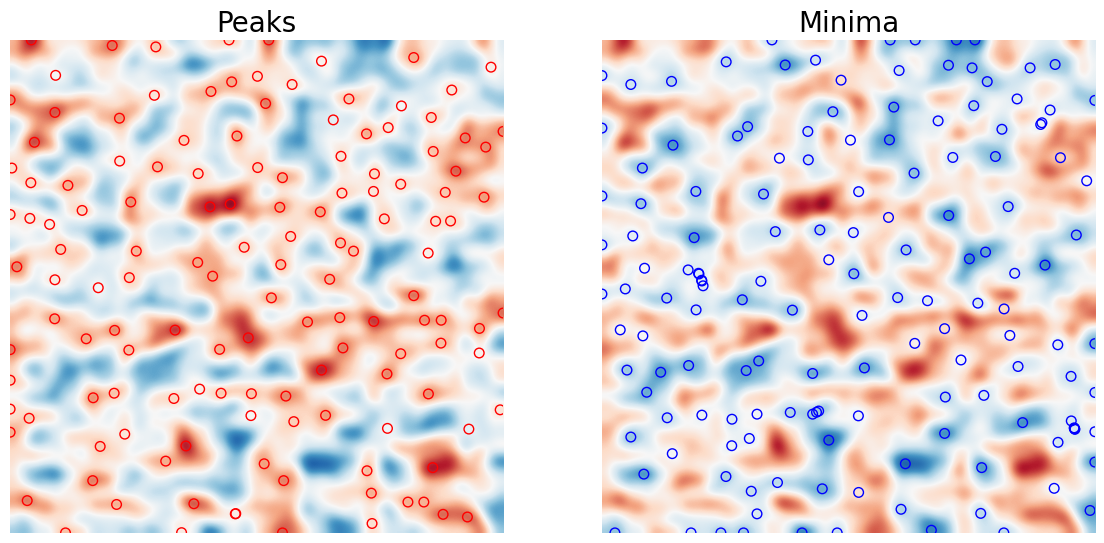
\includegraphics[width=0.8\textwidth]{figures/peaks_minima.png}
    \caption{Identification of peaks and minima in a smoothed convergence map. The left panel shows the smoothed convergence field $\kappa_{\mathrm{smooth}}(\hat{\mathbf{n}})$ with peaks (red circles) satisfying the peak condition (Equation~\eqref{eq:peak_condition}), and the right panel highlights the minima (blue circles) satisfying the minimum condition (Equation~\eqref{eq:min_condition}).}
    \label{fig:peak_min}
\end{figure}

\subsection{Peaks of Gaussian Random Fields}
For a Gaussian random field (GRF), the statistics of peaks and minima can be analytically derived. The expected number density of peaks above a threshold $\nu$ in a GRF is given by:
\begin{equation}
    N_{\mathrm{peak}}(\nu) = \frac{1}{(2\pi)^{3/2} R_*^3} e^{-\nu^2/2} \left[ \nu^2 - 1 \right],
    \label{eq:bbks_peak}
\end{equation}
where $\nu = \tilde{\kappa}_{\mathrm{smooth}}$, and $R_*$ is a characteristic scale defined by:
\begin{equation}
    R_*^2 = \frac{\langle |\nabla \kappa_{\mathrm{smooth}}|^2 \rangle}{\langle \kappa_{\mathrm{smooth}}^2 \rangle}.
    \label{eq:R_star}
\end{equation}
Similarly, the expected number density of minima below $-\nu$ is:
\begin{equation}
    N_{\mathrm{min}}(-\nu) = N_{\mathrm{peak}}(\nu).
    \label{eq:bbks_min}
\end{equation}

\begin{comment}
In particular, the local maxima
and minima on convergence maps are associated with massive haloes
and emptiest regions (voids) in our universe. The study of such
peaks and minima is highly sensitive to non-linear structures and a
complementary probe to constrain S8 (Liu et al. 2015a, b; Kacprzak
et al. 2016; Martinet et al. 2018; Shan et al. 2018; Coulton et al.
2020; Davies et al. 2021; Harnois-Deraps ´ et al. 2021; Davies et al.
2022; Zurcher ¨ et al. 2022; Liu et al. 2023).

measurements of peaks and
minima (Davies et al. 2022; Zürcher et al. 2022; Liu et al. 2023a;
Marques et al. 2024),
\end{comment}


\section{Minkowski Functionals}
\label{sec:minkowski_functionals}
Minkowski functionals are powerful morphological descriptors derived from integral geometry, widely used to quantify the geometry and topology of spatial structures in cosmological datasets. 
Here, we will review \citet{2010PhRvD..81h3505M}, \citet{2012PhRvD..85j3513K} and \citet{2013PhRvD..88l3002P} for a comprehensive understanding of Minkowski functionals and their applications in cosmology.

\subsection{Definition}
Given a two-dimensional random field $\kappa(\hat{\mathbf{n}})$ (in our case, the convergence field) with zero mean and variance $\kappa^2 = \sigma_0^2$, we can consider its excursion sets $\Sigma(\nu) = \{ \kappa > \nu \sigma_0 \}$ which consist of all the points at which the field exceeds a particular threshold value $\nu \sigma_0$. 
Figure~\ref{fig:excursion_sets} depicts the excursion sets $\Sigma(\nu) = \{ \kappa > \nu \sigma_0 \}$ of a two-dimensional convergence field $\kappa(\hat{\mathbf{n}})$, which is characterized by a zero mean and variance $\sigma_0^2$. The figure consists of four panels, each corresponding to an increasing threshold value of $\nu = 0.5, 1, 1.5,$ and $2$. As the threshold $\nu$ increases, the excursion sets progressively diminish in size and connectivity. 
\begin{figure}[ht]
    \centering
    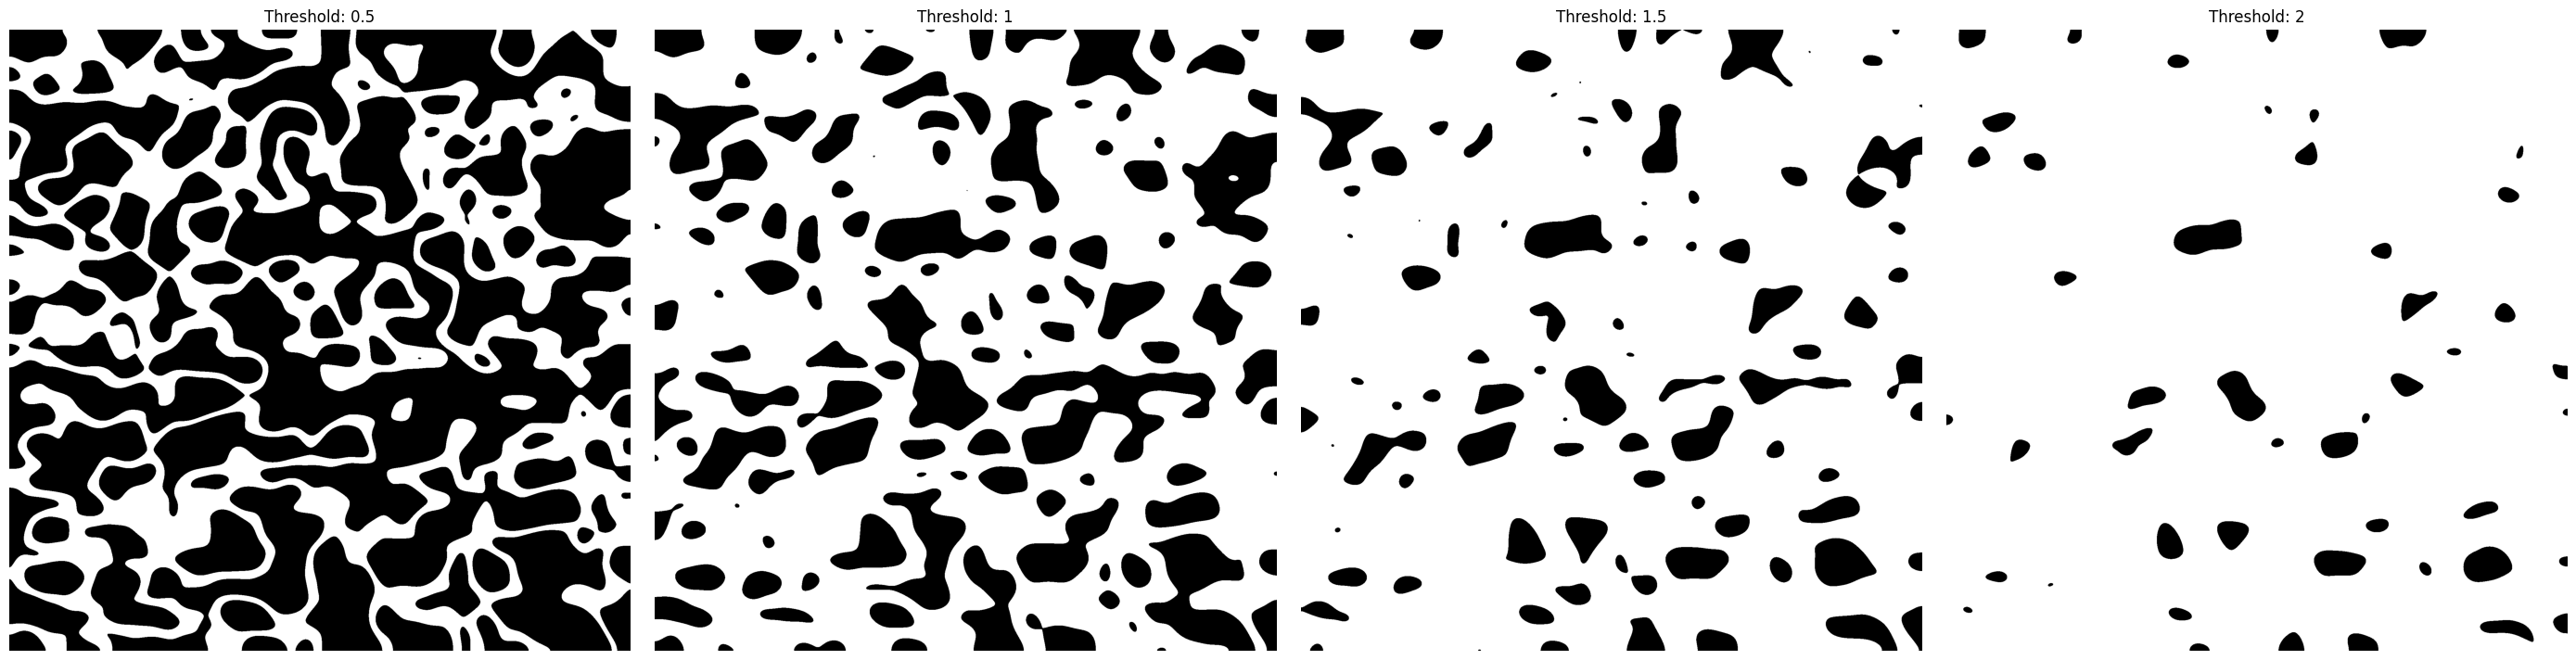
\includegraphics[width=\textwidth]{figures/threshold_comparison.png}
    \caption{Visualization of excursion sets $\Sigma(\nu) = \{ \kappa > \nu \sigma_0 \}$ of a two-dimensional random field $\kappa(\hat{\mathbf{n}})$, where $\kappa$ represents the convergence field with zero mean and variance $\sigma_0^2$. 
    Black regions correspond to regions where the field exceeds the threshold value $\nu \sigma_0$. The panels correspond to increasing threshold values ($\nu = 0.5, 1, 1.5, 2$), illustrating how the size and connectivity of the excursion sets change as the threshold increases.}
    \label{fig:excursion_sets}
\end{figure}
The three Minkowski functionals $V_0(\nu)$, $V_1(\nu)$, and $V_2(\nu)$ measure, respectively, the area, the length of the boundary, and the genus characteristic of these excursion sets:
\begin{align}
    V_0(\nu) &= \frac{1}{A} \int_{\Sigma(\nu)} \, da, \label{eq:minkowski_V0} \\
    V_1(\nu) &= \frac{1}{4A} \int_{\partial \Sigma(\nu)} \, dl, \label{eq:minkowski_V1} \\
    V_2(\nu) &= \frac{1}{2\pi A} \int_{\partial \Sigma(\nu)} \mathcal{K} \, dl, \label{eq:minkowski_V2}
\end{align}
where $A$ is the total area of the field, $da$ and $dl$ are the area and length elements, and $\mathcal{K}$ is the geodesic curvature along the boundary $\partial \Sigma(\nu)$. 

\subsection{Computation of Minkowski Functionals}
In practical applications, Minkowski functionals are computed numerically from discrete convergence maps.

For a given threshold $\nu$, the excursion set $\Sigma(\nu)$ is identified by:
\begin{equation}
    \Sigma(\nu) = \{ \hat{\mathbf{n}} \in S^2 \mid \tilde{\kappa}(\hat{\mathbf{n}}) > \nu \}, \label{eq:excursion_set_normalized}
\end{equation}
where $\tilde{\kappa} = (\kappa - \langle \kappa \rangle) / \sigma_0$ is the normalized convergence field.

Given a pixelized convergence map, the continuous integrals in Equations~\eqref{eq:minkowski_V0}--\eqref{eq:minkowski_V2} are approximated by discrete sums \citep{2012PhRvD..85j3513K}:
\begin{align}
    V_0(\nu) &\approx \frac{1}{N_{\mathrm{pix}}} \sum_{i=1}^{N_{\mathrm{pix}}} \Theta(\tilde{\kappa}_i - \nu), \label{eq:V0_discrete} \\
    V_1(\nu) &\approx \frac{1}{N_{\mathrm{pix}}} \sum_{i=1}^{N_{\mathrm{pix}}}  \delta_D(\tilde{\kappa}_i - \nu) \, \sqrt{\kappa_{, x}^2 + \kappa_{, y}^2}, \label{eq:V1_discrete} \\
    V_2(\nu) &\approx \frac{1}{N_{\mathrm{pix}}} \sum_{i=1}^{N_{\mathrm{pix}}}  \delta_D(\tilde{\kappa}_i - \nu) \, \frac{2\kappa_{, x}\kappa_{, y}\kappa_{, xy} - \kappa_{, x}^2 \kappa_{, yy} - \kappa_{, y}^2}{\kappa_{, xx}{\kappa_{, x}^2 + \kappa_{, y}^2}} \label{eq:V2_discrete}
\end{align}
where $\mathcal{N}(i)$ denotes the set of neighboring pixels to pixel $i$, and $\delta_D$ is the Dirac delta function. The first and second order derivatives $\kappa_{, x}$ etc., are approximated by finite differences.

\subsection{Minkowski Functionals in Gaussian Random Fields}
In the analysis of \emph{Gaussian random fields} (GRFs), Minkowski functionals provide a robust analytical framework for quantifying the morphological characteristics of the field's excursion sets. For a two-dimensional GRF \(\kappa(\hat{\mathbf{n}})\) with zero mean and variance \(\sigma_0^2\), the Minkowski functionals can be explicitly calculated and are given by \citep{2010PhRvD..81h3505M}:
\begin{align}
    V_0(\nu) &= \frac{1}{2}\left[1 - \mathrm{erf}\left( \frac{\nu}{\sqrt{2}\sigma_0} \right) \right], \label{eq:V0_GRF} \\
    V_1(\nu) &= \frac{1}{8\sqrt{2}} \frac{\sigma_1}{\sigma_0} \exp\left( -\frac{\nu^2}{2\sigma_0^2} \right), \label{eq:V1_GRF} \\
    V_2(\nu) &= \frac{\nu}{4\sqrt{2}} \frac{\sigma_1^2}{\sigma_0^3} \exp\left( -\frac{\nu^2}{2\sigma_0^2} \right), \label{eq:V2_GRF}
\end{align}
where \(\nu\) denotes the threshold level defining the excursion set, \(\mathrm{erf}\) is the error function, and \(\sigma_1^2 = \langle |\nabla \kappa|^2 \rangle = \langle \kappa_{, x}^2 + \kappa_{, y}^2 \rangle\) represents the variance of the gradient of the field. Here, \(V_0(\nu)\) corresponds to the area fraction of the excursion set, \(V_1(\nu)\) to the total boundary length per unit area, and \(V_2(\nu)\) to the Euler characteristic per unit area.

\begin{comment}
\subsection{Applications in Cosmology}
Minkowski functionals furnish an algebraic framework for quantifying the geometrical and topological properties of scalar fields \citep{1994A&A...288..697M}. In cosmology, they are instrumental in characterizing the intricate patterns formed by the large-scale structure of the Universe \citep{1996dmu..conf..281S, 1997ApJ...482L...1S}. These patterns, which trace the underlying matter distribution, are sensitive to higher-order statistical moments of the matter density field and thus provide insights beyond those accessible through two-point correlation functions \citep{2001ApJ...551L...5S}.

Recently, Minkowski functionals have been extensively employed in various cosmological investigations. They have been utilized to probe non-linear features in the CMB anisotropies \citep{2012JCAP...01..048L, 2016MNRAS.461.1363N, 2024JCAP...01..039C, 2024JCAP...05..076H}, to analyze anisotropies in the distribution of galaxies \citep{2003PASJ...55..911H, 2022ApJ...928..108A}, to constrain neutrino masses through their impact on the matter power spectrum \citep{2024MNRAS.528.4513M, 2023JCAP...09..037L}, and to test theories of modified gravity that predict deviations from General Relativity on cosmological scales \citep{2017MNRAS.466.2402S, 2024PhRvD.109h3537J}. Moreover, Minkowski functionals have emerged as a powerful and efficient probe for detecting primordial non-Gaussianity, as demonstrated in several studies \citep{2006ApJ...653...11H, 2008MNRAS.385.1613H, 2008MNRAS.389.1439H, 2012MNRAS.425.2187H, 2012ApJ...760...45S}.

In the realm of weak lensing, Minkowski functionals have been proposed as a method to break the degeneracy between the matter density parameter \(\Omega_m\) and the amplitude of matter fluctuations \(\sigma_8\) inherent in traditional two-point statistics \citep{2001ApJ...552L..89M}. Subsequent studies have leveraged Minkowski functionals applied to weak lensing convergence maps to extract cosmological information beyond that accessible through the power spectrum alone, thereby enhancing constraints on cosmological parameters \citep{2012PhRvD..85j3513K, 2013ApJ...774..111S, 2015PhRvD..91j3511P, 2022OJAp....5E..13G}.
\end{comment}

\chapter{Covariance}
\input{background/covariance}

\chapter{Surveys(Make it shorter)}
\section{Introduction to Astronomical Surveys}

\subsection{Purpose and Scientific Objectives}
Contemporary astronomical surveys constitute extensive and systematic observational endeavors designed to map and catalog vast regions of the sky with unparalleled depth and precision. These surveys yield comprehensive datasets that are crucial for addressing fundamental questions in astrophysics and cosmology. They facilitate investigations into the elusive nature of \emph{dark energy}, provide rigorous tests of the \emph{standard cosmological model}—the $\Lambda$CDM paradigm—and enable detailed studies of the formation and evolution of \emph{cosmic structures}. By delivering high-fidelity observational data, these surveys significantly advance our understanding of the Universe and the fundamental physical laws that govern it.

\paragraph{Testing the Standard Cosmological Model}
One of the primary objectives of astronomical surveys is to rigorously test the standard cosmological model, known as the $\Lambda$CDM model (Lambda Cold Dark Matter). While the $\Lambda$CDM model successfully accounts for a wide range of cosmological observations~\cite{Planck2018}, it encounters notable challenges such as the \emph{Hubble tension}—a significant discrepancy between measurements of the Universe's expansion rate derived from early-universe observations~\cite{Planck2018} and those obtained from late-universe observations~\cite{Riess2019}—and inconsistencies in parameters like the amplitude of matter clustering, denoted by $S_8$~\cite{Heymans2021}. These surveys endeavor to produce precise measurements of cosmological parameters, aiming to either corroborate the $\Lambda$CDM model or uncover deviations that could indicate new physics beyond the current paradigm. By juxtaposing high-precision observational data with theoretical predictions, astronomical surveys enhance our understanding of the fundamental forces and constituents that shape the cosmos.

\paragraph{Studying the Growth and Evolution of Cosmic Structures}
Another fundamental objective of astronomical surveys is to investigate the formation and evolution of cosmic structures, including galaxies, galaxy clusters, and dark matter halos. By mapping the spatial distribution of millions of galaxies, these surveys construct detailed maps of dark matter over vast cosmological volumes. Techniques such as \emph{weak gravitational lensing}—which measures subtle distortions in the shapes of background galaxies caused by the gravitational potential of intervening mass distributions—illuminate the role of dark matter in the process of structure formation~\cite{Bartelmann2001}. Moreover, \emph{galaxy-galaxy lensing}, which correlates the lensing signal with the positions of foreground galaxies, provides insights into the connection between luminous matter and the underlying dark matter distribution~\cite{Mandelbaum2017}. These comprehensive maps enable stringent tests of theoretical predictions from various cosmological models regarding the large-scale structure of the Universe.

\subsection{Imaging vs.\ Spectroscopic Surveys}
Astronomical surveys can be broadly categorized into \emph{imaging surveys} and \emph{spectroscopic surveys}, each employing distinct methodologies to capture and analyze celestial phenomena.

\subsubsection{Imaging Surveys}
Imaging surveys acquire wide-field images of the sky across multiple wavelengths, providing spatial data that enable astronomers to map cosmic structures, identify transient events, and analyze galaxy populations. By systematically scanning large regions of the sky, these surveys generate extensive catalogs documenting object positions, apparent magnitudes, and morphological characteristics. The varying depths and angular resolutions of these surveys facilitate the detection of both nearby and distant astronomical objects, thereby supporting detailed morphological and statistical studies across cosmic time. Prominent examples of imaging surveys include the \textit{Sloan Digital Sky Survey} (SDSS; \citealt{2019BAAS...51g.274K}), the \textit{Dark Energy Survey} (DES; \citealt{2018ApJS..239...18A}), and the forthcoming \textit{Legacy Survey of Space and Time} (LSST; \citealt{2019ApJ...873..111I}).

\subsubsection{Spectroscopic Surveys}

Spectroscopic surveys collect detailed spectral data from individual celestial objects by dispersing their emitted light into constituent wavelengths, thereby revealing redshifts, chemical compositions, and kinematic properties. These measurements are indispensable for studying galaxy dynamics, the distribution of dark matter, and the expansion history of the Universe. Unlike imaging surveys that capture broad swaths of the sky, spectroscopic surveys often target specific objects identified in imaging data, focusing on obtaining high-resolution spectral information. The spectral resolution and wavelength coverage are critical parameters that determine the precision of measurements such as redshift determinations and elemental abundances. Key spectroscopic surveys include the \textit{Baryon Oscillation Spectroscopic Survey} (BOSS; \citealt{2013AJ....145...10D}), which investigates baryon acoustic oscillations, the \textit{Dark Energy Spectroscopic Instrument} (DESI; \citealt{2016arXiv161100036D}), designed to map large-scale cosmic structure, and the \textit{Kilo-Degree Survey} (KiDS; \citealt{2013Msngr.154...44D}) with its spectroscopic extensions that enhance research on dark matter and dark energy.

\subsection{Ground-Based vs.\ Space-Based Surveys}

The operational platform of an astronomical survey—whether ground-based or space-based—fundamentally determines its observational capabilities, including wavelength coverage, angular resolution, and sensitivity.

\subsubsection{Ground-Based Surveys}
Ground-based surveys utilize telescopes located on Earth's surface, capitalizing on accessible infrastructure and enabling routine maintenance and upgrades of large, high-power instruments. These observatories can host a diverse array of instruments designed for observations across multiple wavelengths and facilitate prompt follow-up observations. However, atmospheric effects such as absorption, scattering, and turbulence degrade image quality and restrict observations at certain wavelengths, particularly in the ultraviolet and infrared regions. Notable ground-based surveys include the \emph{Hyper Suprime-Cam} (HSC; \citealt{2018PASJ...70S...4A}), the \emph{Dark Energy Survey} (DES; \citealt{2018ApJS..239...18A}), and the \emph{Kilo-Degree Survey} (KiDS; \citealt{2013Msngr.154...44D}).

\subsubsection{Space-Based Surveys}
Space-based surveys operate from satellites or space telescopes positioned above Earth's atmosphere, offering exceptional clarity and sensitivity across a wide range of wavelengths, especially in the ultraviolet and infrared bands that are largely inaccessible from the ground. Free from atmospheric distortions, these instruments achieve high angular resolution and can detect faint, distant objects through long-duration, stable observations. Despite these advantages, space missions are costly, require extensive international collaboration, and present limited opportunities for maintenance, upgrades, or repairs. Prominent examples include the \emph{Hubble Space Telescope} (HST; \citealt{2001ApJ...553...47F}), the forthcoming \emph{Nancy Grace Roman Space Telescope} (\emph{Roman}; \citealt{2015arXiv150303757S}), and the \emph{Gaia} mission~\citep{2016A&A...595A...2G}.

\subsection{Stage-III vs.\ Stage-IV Surveys}
\label{sec:survey-stages}

The classification of astronomical surveys into \emph{Stage-III} and \emph{Stage-IV} categories serves to distinguish successive generations based on technological sophistication, scale, and scientific objectives. While this framework is particularly pertinent in dark energy research~\cite{2006astro.ph..9591A}, it is broadly applicable across cosmology and astrophysics.

\subsubsection{Stage-III Surveys}
Stage-III surveys represent the current generation of large-scale astronomical projects, integrating advanced yet moderately scaled instrumentation and methodologies. Their primary aims include refining cosmological parameters, mapping large-scale structures, and deepening our understanding of dark energy and dark matter. Utilizing multi-band imaging and spectroscopy, Stage-III surveys achieve moderate sky coverage and depth, supported by sophisticated data processing pipelines capable of handling substantial datasets. Notable examples of Stage-III surveys include the \emph{Dark Energy Survey} (DES; \citealt{2018ApJS..239...18A}), the \emph{Kilo-Degree Survey} (KiDS; \citealt{2013Msngr.154...44D}), and the \emph{Hyper Suprime-Cam} survey (HSC; \citealt{2018PASJ...70S...4A}), all of which have provided high-quality data instrumental in advancing cosmological models.

\subsubsection{Stage-IV Surveys}
Stage-IV surveys represent the forthcoming generation of astronomical initiatives, characterized by unparalleled scale, depth, and precision. Leveraging cutting-edge technologies, these surveys aim to achieve high-precision cosmological measurements, explore dark energy and dark matter with greater fidelity, and uncover new astrophysical phenomena. They are distinguished by ultra-wide sky coverage, deep imaging and spectroscopy, high angular resolution, and the integration of multi-wavelength data. Advanced data management techniques are employed to process petabyte-scale datasets efficiently. Prominent examples include the \emph{Legacy Survey of Space and Time} (LSST) conducted by the Vera C.\ Rubin Observatory~\cite{2019ApJ...873..111I}, the \emph{Dark Energy Spectroscopic Instrument} (DESI; \citealt{2016arXiv161100036D}), and the forthcoming \emph{Nancy Grace Roman Space Telescope} (\emph{Roman}; \citealt{2015arXiv150303757S}), all of which are poised to transform our understanding of the cosmos and address critical questions in astrophysics.

\section{Subaru Hyper Suprime-Cam}

\subsection{Instrument Overview}

The \emph{Subaru Hyper Suprime-Cam} (HSC; \citealt{2018PASJ...70S...1M}) is a state-of-the-art wide-field imaging instrument mounted at the prime focus of the 8.2-meter Subaru Telescope located on Maunakea, Hawaii. The HSC features an expansive $1.5^\circ$ diameter field of view, achieved through an array of 104 charge-coupled devices (CCDs), each with $2048 \times 4096$ pixels, culminating in a total of approximately 870 megapixels. This sophisticated configuration enables the acquisition of high-fidelity, wide-field optical data, augmented by a precision corrector lens system that preserves image quality across the entire observational field. The substantial field of view, combined with Subaru's significant light-collecting capabilities, renders the HSC exceptionally well-suited for deep and wide imaging surveys that are critical for studies of \emph{weak gravitational lensing} and the \emph{large-scale structure} of the Universe.

The instrument is equipped with five broad-band filters—\textit{g}, \textit{r}, \textit{i}, \textit{z}, and \textit{y} (\citealt{2018PASJ...70...66K})—alongside several narrow-band filters that cover optical to near-infrared wavelengths. Benefiting from the exceptional atmospheric conditions at Maunakea and the high-resolution optics of the Subaru Telescope, the HSC achieves a median seeing of $0.6$ arcseconds in the $i$-band, facilitating detailed and precise astronomical analyses.

\subsection{Survey Design: The Hyper Suprime-Cam Subaru Strategic Program}

The \emph{Hyper Suprime-Cam Subaru Strategic Program} (HSC-SSP; \citealt{2018PASJ...70S...4A}) is a comprehensive, multi-band imaging survey that exploits the advanced capabilities of the HSC instrument. Initially allocated 300 observing nights over a five-year period starting in March 2014, the program's duration was extended to 340 nights to compensate for observational losses due to weather conditions, technical issues, and seismic activity. The HSC-SSP is meticulously designed to address a broad spectrum of astrophysical inquiries, including but not limited to cosmology, galaxy evolution, and solar system science.

The survey is stratified into three distinct layers, each engineered to achieve specific scientific objectives through varying degrees of sky coverage and imaging depth:

\begin{itemize}
    \item \textbf{Wide Layer}: Encompassing approximately 1,400 square degrees around the celestial equator, the Wide layer attains a depth of $i \sim 26$ magnitudes. This extensive coverage is optimized for mapping large-scale structures and conducting statistical studies of weak gravitational lensing, thereby contributing significantly to our understanding of dark matter distribution and cosmic acceleration.

    \item \textbf{Deep Layer}: Covering roughly 28 square degrees across four distinct fields, the Deep layer reaches a depth of $i \sim 27$ magnitudes. This intermediate configuration balances area and depth, supporting research on galaxy evolution, supernova detection, and the statistical properties of faint astronomical objects.

    \item \textbf{UltraDeep Layer}: Targeting two fields that collectively cover 3.5 square degrees, the UltraDeep layer achieves an impressive depth of $i \sim 28$ magnitudes. Utilizing both broad-band and narrow-band filters, this layer is dedicated to probing the high-redshift Universe, facilitating investigations into early galaxy formation, quasars, and the epoch of reionization, thereby providing critical insights into the early phases of cosmic evolution.
\end{itemize}

\subsection{Data Releases and Processing}

To date, the HSC-SSP has disseminated several public data releases—DR1, DR2, and DR3 (\citealt{2018PASJ...70S...8A, 2019PASJ...71..114A, 2022PASJ...74..247A})—each incorporating progressively larger datasets, enhanced calibration procedures, and refined data processing methodologies. The data processing pipeline is managed using the \emph{Legacy Survey of Space and Time} (LSST) Science Pipelines, which provide high-quality analysis tools accessible to the astronomical community. These tools generate calibrated imaging data, comprehensive photometric catalogs, and advanced data products such as photometric redshifts and precise shape measurements. Consequently, the HSC-SSP data releases empower a wide array of scientific investigations and promote collaborative advancements within the field of astronomy.

\section{Dark Energy Survey}

\subsection{Overview and Objectives}

The \emph{Dark Energy Survey} (DES; \citealt{2005astro.ph.10346T, 2018ApJS..239...18A, 2021ApJS..255...20A}) was meticulously designed as a comprehensive, wide-field imaging survey operating in optical and near-infrared wavelengths, with the primary objective of probing the nature of cosmic acceleration and the underlying mechanism of \emph{dark energy}. Spanning approximately $5{,}000$ square degrees of the Southern Galactic Cap, DES was conducted over a six-year period from August 2013 to January 2019. The survey utilized the $570$-megapixel \emph{Dark Energy Camera} (DECam; \citealt{2015AJ....150..150F}), which is mounted on the 4-meter \emph{Blanco Telescope} at the Cerro Tololo Inter-American Observatory (CTIO) in Chile.

\subsection{Survey Components}

DES observations were strategically divided into two primary components: the \emph{Wide-Area Survey} and the \emph{Supernova Survey}, each meticulously tailored to address specific scientific goals within the overarching framework of DES.

\subsubsection{Wide-Area Survey}

The Wide-Area Survey constituted the principal observational effort of DES, covering approximately $5{,}000$ square degrees across five photometric bands ($g$, $r$, $i$, $z$, $Y$). This extensive footprint was purposefully selected to overlap with other significant surveys, such as the \emph{South Pole Telescope Survey} and the \emph{Sloan Digital Sky Survey} (SDSS) Stripe 82~\cite{2009ApJS..182..543A}, thereby enhancing calibration accuracy and enabling synergistic cross-survey analyses. The Wide-Area Survey aimed to map the large-scale structure of the Universe with high precision, facilitating studies on galaxy clustering, weak gravitational lensing, and the abundance of galaxy clusters, all of which are sensitive probes of dark energy and cosmological parameters.

\subsubsection{Supernova Survey}

Complementing the Wide-Area Survey, the Supernova Survey focused on a more concentrated region of approximately $27$ square degrees. This component employed a higher observational cadence, with images acquired in the $g$, $r$, $i$, and $z$ bands roughly every seven days. Such a cadence was specifically designed to capture transient phenomena, notably \emph{Type Ia supernovae}~\cite{2019PhRvL.122q1301A}, which serve as standard candles for cosmic distance measurements. By monitoring these supernovae over time, the Supernova Survey aimed to construct a Hubble diagram extending to high redshifts, thereby providing stringent constraints on the equation of state of dark energy.

\subsection{Instrumentation and Data Processing}

DECam, the instrument central to DES, features a focal plane array of 62 science CCDs, each with $2048 \times 4096$ pixels, providing a large field of view of $2.2$ degrees in diameter. The camera's design includes specialized optics to achieve uniform image quality across the field, essential for weak lensing measurements that require precise shape determinations of distant galaxies.

Data processing for DES was handled by the \emph{DES Data Management} (DESDM) system~\cite{2008SPIE.7016E..0LM}, which performed tasks ranging from image detrending and astrometric calibration to co-addition and catalog generation. Advanced algorithms were employed for photometric calibration, object detection, and classification, ensuring high-quality data products suitable for cosmological analyses.

\subsection{Scientific Contributions}

DES has made significant contributions to cosmology and astrophysics, including precise measurements of cosmic shear~\cite{2022PhRvD.105b3514A} and galaxy clustering~\cite{2022PhRvD.105b3520A}. The combination of these probes has led to improved constraints on cosmological parameters, particularly the matter density $\Omega_m$ and the amplitude of matter fluctuations $\sigma_8$. Furthermore, DES data have been instrumental in addressing tensions in cosmological measurements, such as the $S_8$ discrepancy, and in exploring possible extensions to the $\Lambda$CDM model.


\section{Legacy Survey of Space and Time}

\subsection{Overview and Scientific Objectives}

The \emph{Legacy Survey of Space and Time} (LSST; \citealt{2009arXiv0912.0201L, 2019ApJ...873..111I}), conducted by the Vera C.\ Rubin Observatory, is a groundbreaking optical survey meticulously designed to perform a comprehensive imaging campaign covering approximately half of the celestial sphere. Operating with six photometric filters (\emph{ugrizy}), LSST will systematically re-image its surveyed regions at intervals of a few nights over a planned ten-year observational period. This extensive survey is anticipated to produce an unparalleled dataset, comprising approximately $3.2 \times 10^{13}$ individual observations of around $2 \times 10^{10}$ galaxies, along with a comparable number of stellar objects. This vast repository of observations will enable a broad spectrum of scientific investigations, including studies in cosmology, Galactic structure, and time-domain astrophysics.

\subsection{Instrumentation and Survey Strategy}

To achieve its ambitious scientific objectives, LSST has been constructed as an advanced, wide-field observatory centered around an 8.4-meter primary mirror and a field of view spanning 9.6 square degrees. The system's observational capabilities are enhanced by a 3.2-gigapixel camera, facilitating high-throughput data acquisition. The unique optical design employs a three-mirror system to deliver a wide field of view with excellent image quality across the entire focal plane.

The survey primarily employs a \emph{deep-wide-fast} observing strategy, allocating approximately 90\% of the telescope's operational time to this primary mode~\cite{2009arXiv0912.0201L}. This approach aims to maximize both spatial coverage and temporal cadence across the main survey region, enabling the detection of transient phenomena and the mapping of large-scale structures. The remaining 10\% of LSST's observing time is dedicated to specialized programs designed to address specific astrophysical phenomena. These programs include \emph{deep drilling fields}, which involve intensified observations in selected regions to achieve greater depth, and targeted surveys of dynamically complex areas, such as the Galactic plane. These tailored observational approaches are integral to fulfilling LSST's broader scientific mandate, offering critical data to complement the primary survey and enabling detailed analyses of both local and distant astronomical phenomena.

\subsection{Scientific Impact}

LSST is expected to make transformative contributions across multiple domains of astrophysics. In cosmology, it will provide precise measurements of dark energy parameters through studies of weak gravitational lensing, supernovae, baryon acoustic oscillations, and large-scale structure~\cite{2012arXiv1211.0310L}. In the study of the Milky Way, LSST will map the distribution and kinematics of stars, facilitating investigations into the Galaxy's formation history and structure~\cite{2019NatRP...1..450R}. The time-domain capabilities of LSST will enable the discovery and monitoring of transient and variable objects, such as supernovae, variable stars, and potentially hazardous near-Earth objects~\cite{2018Icar..303..181J}. Furthermore, LSST's extensive dataset will be invaluable for probing fundamental physics, such as testing general relativity on cosmological scales and searching for signatures of new physics beyond the Standard Model.

\section{Nancy Grace Roman Space Telescope}

\subsection{Overview and Mission Objectives}

The \emph{Nancy Grace Roman Space Telescope} (hereafter referred to as \emph{Roman}; formerly designated as the \emph{Wide-Field Infrared Survey Telescope}, \textit{WFIRST}; \citealt{2015arXiv150303757S}) represents a seminal endeavor within NASA's astrophysics portfolio. This mission leverages a 2.4-meter aperture telescope, originally developed for national reconnaissance purposes, repurposing its advanced instrumentation and observational capabilities toward forefront astronomical research. The \emph{Roman} mission is designed to address key questions in cosmology and exoplanet science, thereby significantly enhancing our understanding of the Universe's expansion history, the distribution of dark matter and dark energy, and the prevalence of planetary systems in our galaxy.

\subsection{Surveys and Scientific Goals}

The \emph{Roman} Space Telescope's scientific program is anchored by two primary surveys: the \emph{High Latitude Survey} and the \emph{Galactic Bulge Time Domain Survey}, each meticulously designed to achieve specific scientific objectives.

\subsubsection{High Latitude Survey}

A cornerstone of the \emph{Roman}'s scientific agenda is the \textbf{High Latitude Survey}, engineered to probe the enigmatic phenomenon of dark energy, which is hypothesized to drive the accelerated expansion of the Universe~\cite{1998AJ....116.1009R, 1999ApJ...517..565P}. This survey integrates a tripartite observational strategy to examine both the temporal evolution of cosmic expansion and the growth of large-scale structures. The employed methodologies encompass:

\begin{itemize}
    \item \textbf{Supernova Surveys}: Utilizing Type Ia supernovae as standard candles to trace the expansion history of the Universe~\cite{2011ApJ...737..102S}.
    \item \textbf{Weak Gravitational Lensing Imaging}: Mapping the distribution of dark matter through the subtle distortions of background galaxies~\cite{2001PhR...340..291B}.
    \item \textbf{Spectroscopic Surveys of Baryon Acoustic Oscillations}: Measuring the scale of baryon acoustic oscillations to serve as a cosmological standard ruler~\cite{2005ApJ...633..560E}.
\end{itemize}

These techniques collectively furnish a comprehensive understanding of the Universe's expansion history, thereby elucidating the properties and dynamics of dark matter and dark energy. The High Latitude Survey is anticipated to cover thousands of square degrees, providing high-resolution imaging and spectroscopy in the near-infrared wavelengths.

\subsubsection{Galactic Bulge Time Domain Survey}

Complementing the High Latitude Survey, the \textbf{Galactic Bulge Time Domain Survey} employs the microlensing technique to detect and characterize a substantial population of exoplanets, including those with masses as low as that of Mars~\cite{2019ApJS..241....3P}. Focusing on stellar populations within the Milky Way's bulge, this survey enhances our comprehension of planetary formation and distribution mechanisms in environments with high stellar density. By monitoring millions of stars over time, the \emph{Roman} Space Telescope aims to detect the gravitational microlensing events caused by planets orbiting both luminous and dark host stars, thus expanding the demographic census of exoplanets~\cite{2012ARA&A..50..411G}.

\subsection{Instrumentation and Capabilities}

The \emph{Roman} Space Telescope is equipped with a 2.4-meter primary mirror, comparable in size to the \emph{Hubble Space Telescope}, but with a significantly larger field of view—approximately 100 times greater~\cite{2015arXiv150303757S}. The primary instruments include:

\begin{itemize}
    \item \textbf{Wide Field Instrument (WFI)}: A near-infrared imager and spectrometer that provides high-resolution imaging and integral-field spectroscopy over a large field of view.
    \item \textbf{Coronagraph Instrument}: A technology demonstration instrument designed to perform high-contrast imaging and spectroscopy of exoplanets and circumstellar disks.
\end{itemize}

These advanced instruments enable the \emph{Roman} Space Telescope to perform wide-field surveys with unprecedented sensitivity and resolution in the near-infrared regime.

\subsection{Expected Scientific Contributions}

The \emph{Roman} Space Telescope is poised to make transformative contributions to astrophysics and cosmology. In addition to its primary surveys, it will offer opportunities for a \emph{Guest Observer} program, allowing the broader scientific community to propose observations for a wide range of astrophysical phenomena~\cite{2019arXiv190205569A}. The mission is expected to:

\begin{itemize}
    \item Provide precise measurements of cosmological parameters, refining our understanding of dark energy and the geometry of the Universe~\cite{2018ApJ...867...23H}.
    \item Expand the census of exoplanets, particularly those in the outer regions of planetary systems, thereby informing models of planetary formation and evolution~\cite{2019ApJS..241....3P}.
    \item Advance the study of galaxy formation and evolution through deep imaging and spectroscopy of distant galaxies~\cite{2018MNRAS.477.5382B}.
    \item Enhance our understanding of the Milky Way's structure and stellar populations~\cite{2020AJ....160..123J}.
\end{itemize}

By addressing these fundamental questions, the \emph{Roman} Space Telescope will significantly augment our knowledge of the cosmos and lay the groundwork for future astronomical discoveries.


\chapter{Simulations}
\input{numerical}

\chapter{Methods}
\input{methods}

\chapter{Results}
\input{results}

\chapter{Discussion}
\input{discussion}

% \chapter{Conclusions and Future Work}
% \section{Summary of Key Findings}
% This thesis demonstrated the importance of accounting for artefacts in weak lensing simulations to improve covariance matrix estimations.

% \section{Limitations and Future Work}
% Future research could explore more complex simulations and apply findings to LSST and Roman surveys.

% \appendix  % Start of appendices

% \chapter{Additional Mathematical Derivations}
% Here you can include detailed derivations that were omitted from the main text.

\bibliographystyle{mnras}
\bibliography{thesis_bib.bib}

\end{document}